\chapter{State of the Art}
\label{lab:sota}
As already mentioned in section \ref{sec:terms}, \textit{Development}, developing software is greatly facilitated using existing building blocks instead of writing the entirety of program code from scratch. Especially Web server applications benefit from \textit{frameworks} -- i.e. third-party software that can be extended with application-specific code -- because frameworks generally provide support for standard, repetitive procedures like handling network communication, database access, caching\footnote{The \textit{cache} is mainly short-lived memory used for faster delivery of dynamic data.} and URL mapping\footnote{URL mapping is the process of deciding which action should be taken based on the requested network URL.}. The process of minimising repetitive code and maximising code reusability can be described as reducing \textit{boilerplate code} or by the slogan \textit{DRY}\footnote{Don't repeat yourself} \cite[p. 149]{Scala} \cite[p. 1]{Orsini2008}.

On the other hand, modern Web frameworks often include ways of abstracting concurrency or build on existing concurrency frameworks themselves. This can save the developer from having to deal with low-level concerns like thread scheduling and message passing (see section \ref{sec:threads} and \ref{lab:actormodel}, respectively). \textit{Full-stack} Web frameworks often handle many -- if not all -- tasks common to specific networking applications. They may even include their own Web server to improve the handling of numerous concurrent requests. Figure \ref{fig:full_stack} gives a brief overview of typical full-stack framework capabilities. 

\begin{figure}
\centering\small
\setlength{\tabcolsep}{0mm}
  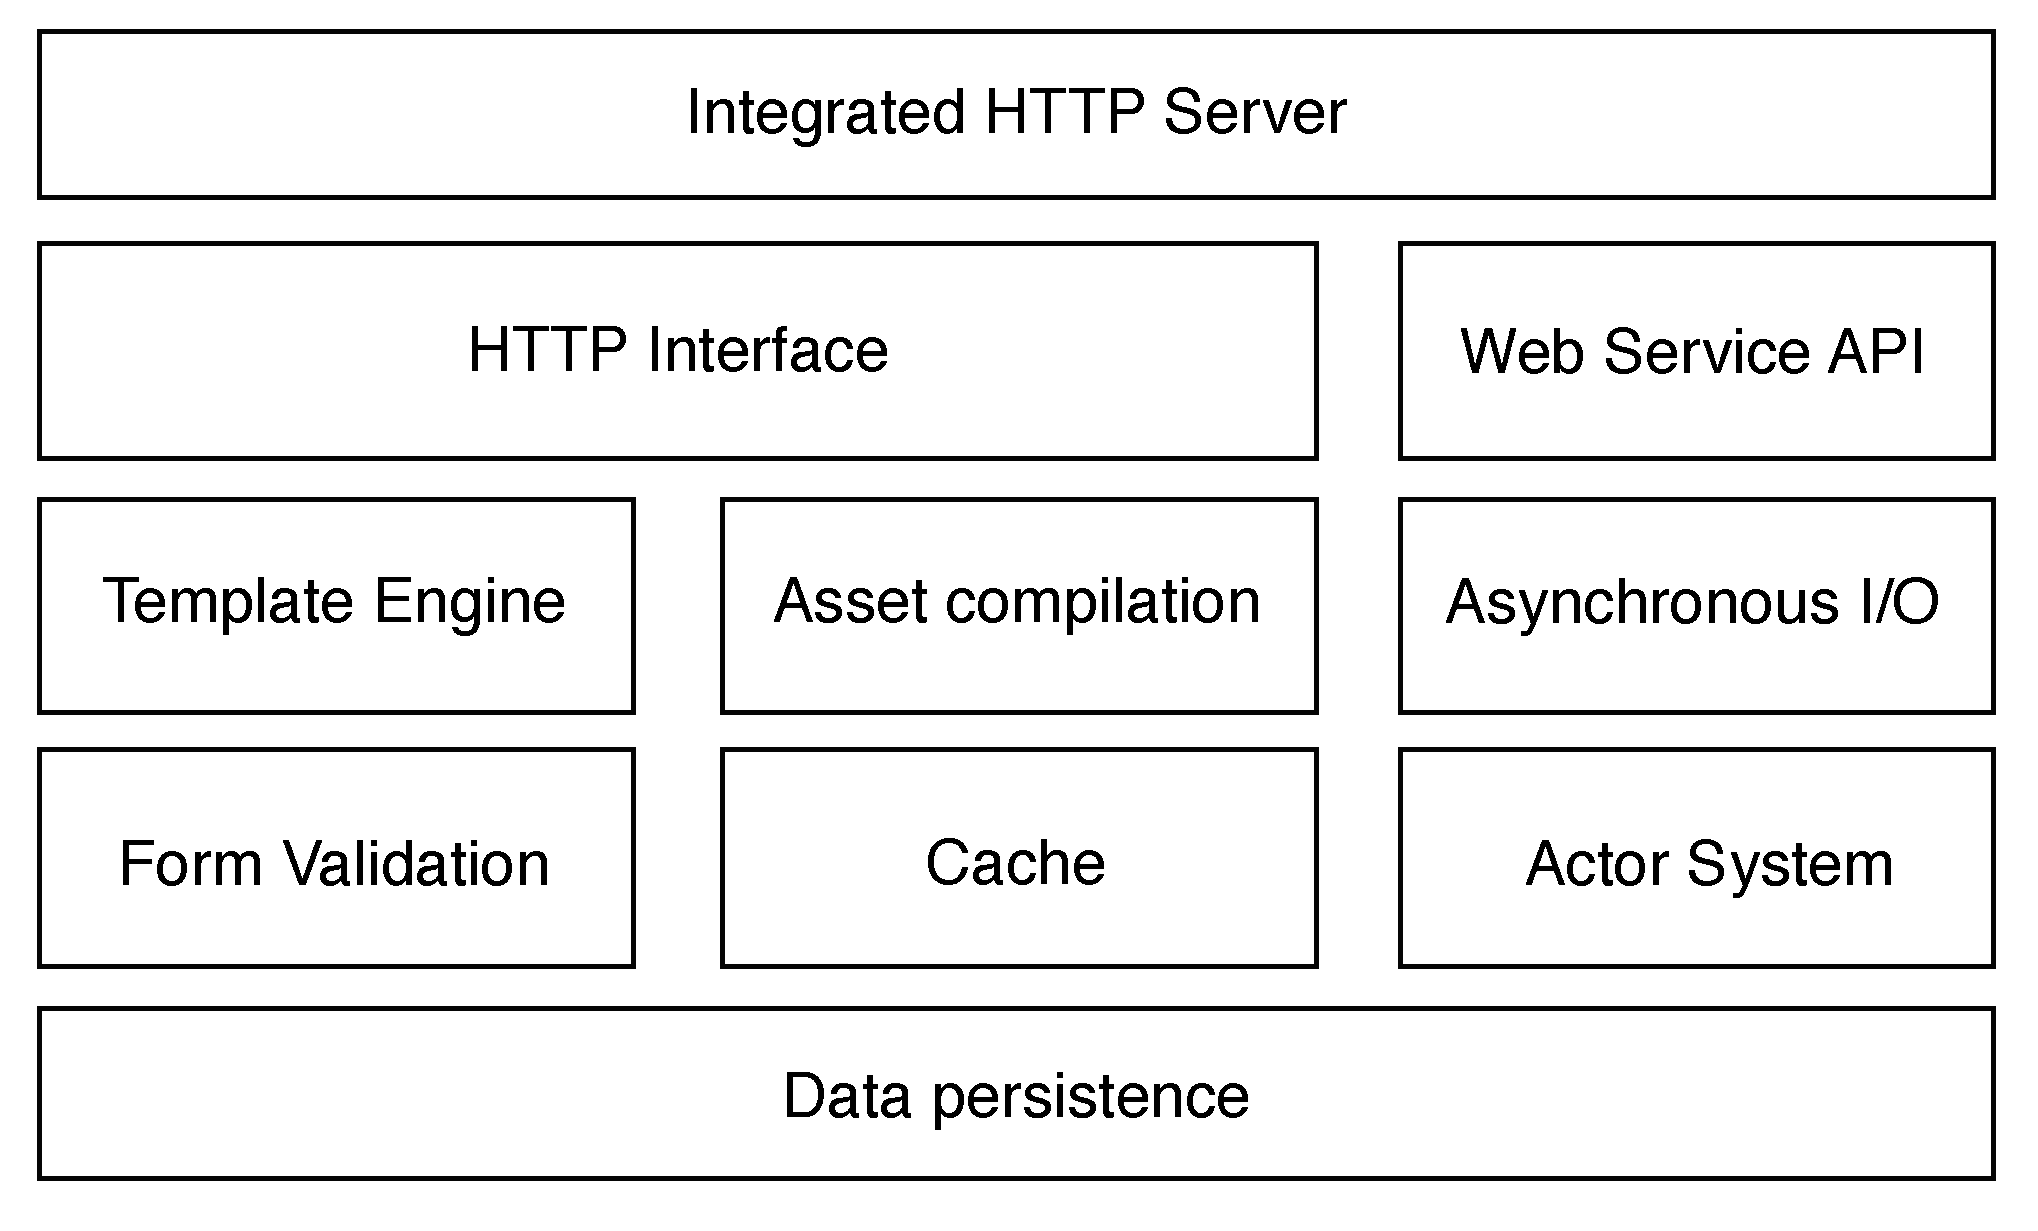
\includegraphics[width=.90\textwidth]{full_stack}
\caption{
A Web framework aims to facilitate development by including frequently used capabilities. Inbound and outbound network communication represents a large share of common features (top three elements). Also, served assets like websites and images play a role in certain use-cases (but do not in case of a purely API-focussed server). Storage in form of cache and data persistance is also important for most applications. However, asynchronous I/O and Event- and Actor-based interfaces are the main focus of this chapter. Image based on the structure of the \textit{Play! Framework} (\url{http://www.playframework.com}) \cite{Scala}
}
\label{fig:full_stack}
\end{figure}

This chapter presents selected approaches to performance-critical event-based and actor-based concurrency abstraction with respect to the criteria defined in section \ref{sec:terms} and taking into account the technical issues elaborated in section \ref{sec:concurrency}.

\section{Event-based technologies}

\subsection{Node.js}

\textit{Node.js}\footnote{\url{http://nodejs.org/}} is not only a framework, but rather a dedicated open source software platform for purely event-driven applications. User-level code is written in \textit{JavaScript} and interpreted by the \textit{V8}\footnote{\url{https://code.google.com/p/v8/}} engine also used in the \textit{Google Chrome}\footnote{\url{https://www.google.com/intl/en/chrome/browser/}} Web browser \cite[p. 19]{Hughes-Croucher2012}. This is reasonable since \textit{JavaScript} was originally used primarily for programming client-side website behaviour; however, Node.js uses a module system\footnote{Using the \textit{CommonJS} module specification (\url{http://www.commonjs.org/})} to add various Web server-specific features. These features include -- among others -- networking abstractions, file and operating system abstractions and replication and scheduling utilities\footnote{See \url{http://nodejs.org/api/} for an exhaustive list of system modules or \url{https://www.npmjs.org/} for a popular extension module repository}. The platform also includes its own Web server via the \texttt{http} module.

\subsubsection*{Development}
\label{lab:nodehttp}
Program modules are represented by \textit{JavaScript} files. The entry point of a program must be defined by specifying the main \textit{JavaScript} file upon application launch \cite[p. 16]{Hughes-Croucher2012}. To use a module it has to be included with the \texttt{require} command. Program flow typically propagates via callbacks (see section \ref{lab:flow}). An example of these concepts can be seen in program \ref{prog:node-http}.

\begin{program}
  \caption{This example illustrates the concepts introduced at the beginning of section \ref{lab:nodehttp}. In line 1, a HTTP network abstraction is loaded and exported to a variable for later use. Line 2 calls a function on this variable, requesting the creation of a new server instance; this function takes as parameter an \textit{anonymous} callback function (meaning that it is passed directly in form of a function rather than as an assigned variable), which is called upon each incoming HTTP request. The function's two parameters are handles to the HTTP request and response, respectively. Line 3 and 4 generate the response by setting the HTTP status code, the \texttt{Content-Type} header and the response body. The server is started via the function \texttt{listen}, which accepts a network port and IP address. Code source: \cite[p. 9]{Hughes-Croucher2012}}
  \label{prog:node-http}
  \begin{JavaCode}
var http = require('http');
http.createServer(function (req, res) {
    res.writeHead(200, {'Content-Type': 'text/plain'}); 
    res.end('Hello World\n');
}).listen(8124, "127.0.0.1");
console.log('Server running at http://127.0.0.1:8124/');
  \end{JavaCode}
\end{program}

Due to the functional nature of \textit{JavaScript}, callback functions can be the main driving force of asynchronous program flow. The following factors support this \cite{node-loop}:
\begin{itemize}
  \item First-class functions can be handled like any other data type; they can be stored in variables, passed as parameters and executed when needed.
  \item Functions can be composed of multiple \textit{anonymous} functions, which allows for flexible ordered execution (as seen in program \ref{prog:node-http}).
\end{itemize}

However, there are several caveats to exclusively callback-driven program flow. For one, multiple callbacks executed sequentially are not guaranteed to return in a certain order. There is also no predefined way of awaiting multiple callback results. Also, callbacks -- when used excessively -- tend to lead to quite unreadable code and, ultimately, to a condition known as the \textit{Pyramid of Doom} (see program \ref{prog:doom}).

\begin{program}
  \caption{Multiple dependent callback functions can lead to a structure called \textit{Pyramid of Doom}, which can impede code readability. Every step function (i.e. \texttt{step1}, \texttt{step2}, \ldots) asynchronously depends on the result of the previous one. In this example, code indentation tends to increase faster than line progression. Code source: \cite[p. 21]{Torstensson2012}}
  \label{prog:doom}
  \begin{JavaCode}
step1(function (value1) {
    step2(value1, function (value2) {
        step3(value2, function (value3) {
            step4(value3, function (value4) {
                // Do something with value4
            });
        });
    });
});	
  \end{JavaCode}
\end{program}

To relieve these problems, the \textit{promise} paradigm can be used as an abstraction for callbacks. With a promise framework like the one included in the popular \textit{jQuery} library\footnote{\url{http://jquery.com/}} or the \textit{Q} library\footnote{\url{https://github.com/kriskowal/q}}, sequential functions can be written more idiomatically as a chain of commands (see program \ref{prog:promises}). When a promise is created, the result is \textit{deferred}, i.e. returned at a later point in time. If the action of the promise was successful, the promise is \textit{resolved}, otherwise it is \textit{rejected}. There is also a comprehension that allows for resolving multiple promises in parallel and treating the results as a single array of values as soon as all promises are resolved:

\begin{JavaCode}
Q.all([stepA, stepB]).then(function (results) {
    var resultA = results[0];
    var resultB = results[1];
});
\end{JavaCode}

\begin{program}
  \caption{By using a promise library, sequential asynchronous processing can be simplified. The \texttt{then} function accepts a first-class callback function and, optionally, an error handler (as seen in line 7). Code source: \cite[p. 21]{Torstensson2012}}
  \label{prog:promises}
  \begin{JavaCode}
step1()
.then(step2)
.then(step3)
.then(step4)
.then(function (value4) {
    // Do something with value4
}, function (error) {
    // Handle any error from step1 through step4
})
  \end{JavaCode}
\end{program}

Another means of program flow in \textit{JavaScript} is via explicit events. In \textit{Node.js}, this can be conveniently done by using the \texttt{events} module. New events are created and handled by an instance of \texttt{EventEmitter} (see program \ref{prog:emitter}). This way, a very flexible (yet \textit{flat}, see section \ref{lab:flow}) program flow can be realised.

\begin{program}
  \caption{A simple example of explicit events. First, the emitter created through the \texttt{events} module registers a behaviour (in form of a callback function) for a certain event type (i.e. \texttt{doorOpen}). At an arbitrary point in time an event of this type is created and triggers the callback function. Code source: \cite{Cogneau2013}}
  \label{prog:emitter}
  \begin{JavaCode}
var events = require('events');
var eventEmitter = new events.EventEmitter();
 
var ringBell = function ringBell()
{
    console.log('ring ring ring');
}
eventEmitter.on('doorOpen', ringBell);
 
eventEmitter.emit('doorOpen');
  \end{JavaCode}
\end{program}

The \texttt{async}\footnote{\url{https://github.com/caolan/async}} module provides a number of functions that abstract and simplify working with asynchronous actions in a functional way and has an even wider scope than the \textit{Q} library. For instance, it introduces comprehensions to apply an asynchronous function to multiple values (\texttt{each()}) and facilitates control flow with helpers for serial and parallel execution:

\begin{JavaCode}
async.parallel([
    function(){ ... },
    function(){ ... }
], callback);
\end{JavaCode}

Independent of the exact method of implementing concurrency in \textit{Node.js}, \textit{inversion of control} (see section \ref{lab:events}) plays a big role and its drawbacks (e.g. reduced code readability) are hard to avoid without using special libraries \cite[p. 93]{Erb2012}. However, because \textit{JavaScript} is a very popular language due to its use in website development, the adoption rate and the enthusiasm event of less experienced developers help with building a rich ecosystem around the platform \cite[p. 27]{Hughes-Croucher2012}.

\textit{Node.js} applications can also benefit from certain framework modules that add \textit{MVC} (Model-View-Controller) capabilities. One such module is the \textit{express} framework\footnote{\url{http://expressjs.com/}}, which includes features such as advanced routing and templates and brings \textit{Node.js} one step closer to being a full-stack Web framework (see section \ref{lab:sota}).

\subsubsection*{Scalability}
In the previous section, methods of implementing asynchronous behaviour in \textit{Node.js} applications were listed. This section aims to explain the implications of executing this applications with regard to the execution environment.

Applications running on \textit{Node.js} per default only use a single thread for processing \cite{node-loop}. As mentioned in the previous chapter, this has a positive effect on scheduling overhead. Because of the nature of \textit{JavaScript} and \textit{Node.js} (e.g. asynchronous networking and file abstractions, use of callbacks), it is comparably easy to write code that does not block the processing thread. However, \textit{if} blocking occurs, the consequence is that the whole application is unable to process any requests until the blocking action has finished. On the other hand, this removes any need for synchronisation concerns and prevents address space conflicts between threads \cite[p. 105]{Erb2012}.

To scale out a \textit{Node.js}-based application, two main steps can be taken: Just scaling out on a single multi-core machine or scaling out on multiple machines. The first can be archived by creating multiple instances of the same program using the \texttt{cluster} module of \textit{Node.js} (see program \ref{prog:cluster}). This way, a master process has control over several child processes that handle requests asynchronously based on load balancing \cite[p. 64]{Hughes-Croucher2012}. The technique of having one process create child instances is called forking. If forking is not supported by the operating system (e.g. on Windows systems), the application creates multiple threads in the same process. Running the application on multiple servers has no special implications for \textit{Node.js}; shared state has to be archived by a messaging protocol like \textit{pub-sub} \cite[p. 137]{Hughes-Croucher2012}.

\begin{program}
  \caption{The \texttt{cluster} module provides an abstraction of creating multiple instances of program execution. The first process running the code is defined as the master process and all other processes (the number of processes depends on the number of processing cores in the system) are forked as child processes. Code source: \cite{Hughes-Croucher2012}}
  \label{prog:cluster}
  \begin{JavaCode}
var cluster = require('cluster'); 
var http = require('http');
var numCPUs = require('os').cpus().length;

if (cluster.isMaster) {
    // Fork workers.
    for (var i = 0; i < numCPUs; i++) {
        cluster.fork();
    }
    ...
} else {
    // Worker processes have a http server.
    http.Server(function(req, res) {
        res.writeHead(200);
        res.end("hello world\n");
    }).listen(8000);
}
  \end{JavaCode}
\end{program}

\subsubsection*{Performance}
\textit{Node.js} is very suitable for massive connection concurrency and data-heavy applications \cite[p. 44]{Torstensson2012}. The \textit{V8} engine executes \textit{JavaScript} code at a very favourable speed; interfaces that often slow down browser-based applications (like the \textit{DOM}(Document Object Model)) are not present in a server-side environment. However, the code is executed by interpretation, which is inherently slower than the execution of binary files or virtual machine bytecode (like \textit{Java}). Figure \ref{fig:node_performance} illustrates the serious impact of intensive computations on response time. 

\begin{figure}
\centering\small
\setlength{\tabcolsep}{0mm}
  \includegraphics[width=.80\textwidth]{node_performance}
\caption{
In this figure taken from a performance analysis of D. Torstensson and E. Eloff, requests are sent to a \textit{Node.js} server with different payload sizes. The requests are sent both with and without authentication; authentication is done by hashing (i.e. processing) the whole payload using the \textit{SHA1-HMAC} algorithm. Larger payloads are more computationally intensive and result in a longer response time. Image source: \cite{Torstensson2012}
}
\label{fig:node_performance}
\end{figure}

\subsection{Eventmachine}
Ruby\footnote{\url{https://www.ruby-lang.org}} is a dynamic programming language that has a high adoption rate due to the popular \textit{Ruby on Rails} MVC framework that powers a lot of modern Websites \cite[p. 11]{Orsini2008}. In contrast to \textit{JavaScript}, \textit{Ruby} does not support event-driven programming by nature.


Fibers


\subsection{Others}
React, Derby, Twisted, Java NIO

\section{Actor-based technologies}

\subsection{Play!} \newpage a \newpage a \newpage a \newpage a \newpage a
The Scala Actor Model


\subsection{Lattice} \newpage a \newpage a

vs rails

\subsection{Others}
Lift











































